\newpage\null\thispagestyle{empty}\newpage
\clearpage{\thispagestyle{empty}\cleardoublepage}
\part{Software}
% \acbarrier
\parttoc
% 
% 
% 
\setcounter{chapter}{3}
\chapter{Nerve fiber modelling}
\label{chap:sof:modelling}
% 
In \cref{chap:neuro} both the structure of nerve fibers and the macroscopic structure of \ac{WM} were described.
The question is how to represent such a structure in a computer algorithm?
For simple fiber configurations, \eg{} parallel, linear nerve fibers, this is quite straightforward.
However, it has been shown that irregular, non-symmetric nerve fiber configurations are necessary to obtain a realistic result for microscopy simulations based on the wave nature of the light \cite{MenzelDissertation}.
Therefore one needs ideally a representation, which allows to build any kind of pattern.
\par
%
Many solutions are already available.
A common one is used in graphical visualizations.
A rope or fiber, \ie{} a raw object, is defined by a trajectory with a radius.
From this, a surrounding mesh is generated.
In visualization, the mesh is used to apply textures to represent a surface.
Such meshes are \eg{} used in Monte Carlo simulations of \ac{dMRI} \cite{Ginsburger2019,ginsburgerDis2019}.
In this type of simulation, the meshes help calculate whether a water molecule travels through the surface of a nerve fiber, i.e., the surface of the mesh.
However, this representation is very computationally intensive because the number of triangles that must be present in the mesh is quite high.
\par
%
When creating complex nerve fiber structures, it is even more important that the nerve fibers do not overlap.
In simulations in which the wave nature of light is modeled, this otherwise leads to significantly altered results.
To achieve this, either the user must define such a structure in advance, or a computer algorithm must build such structures from input parameters.
Considering the immense number of configuration possibilities that nerve fibers can have even in a small volume, the task is almost impossible for a user to solve except for trivial configurations.
The same is true for a computer algorithm.
One could write an algorithm that defines a single fiber in a volume and then places the next one, making sure that none overlaps and so on.
This works well up to a point.
Even if an algorithm always finds a solution to find a path through an partially filled volume, at some point the volume will appear to be full, but still have plenty of free space between fibers.
Of course, one can minimize this behavior by trying to place nearly parallel fibers, but again, looking at real tissue data, \eg{} \cref{fig:brainTPFM, fig:elecMic}, this does not reflect reality.
Even in a fiber bundle, the fibers are so densely packed that you can't just add another fiber in a way that wastes volume over time (\ie{} add more fibers).
\par
%
The solution found in this work is to allow the placement of nerve fibers in any way and without any restriction.
However, the overlap must then be removed.
The idea is quite simple.
Check all fibers for collisions with each other.
If a collision occurs, try to remove it by moving the colliding parts slightly away from each other.
Repeat this step until all collisions are removed.
\par
%
This idea \cite{Matuschke2019} with all its necessary prerequisites is described in detail in the following chapter.
First, the representation of a nerve fiber is defined in a way that it already takes into account to be as performant as possible for the collision process.
Then, additional \textit{building} functions are designed to help the user quickly define a volume with nerve fibers.
Finally, the solution algorithm for resolving the collisions with its parallel components is explained in detail.
In addition, another approach based on this idea and developed in this work with colleagues from \ac{dMRI} is explained in detail.
This one focuses on the placement of neurons such as astrocytes or olegodendrocytes with their (arms) in the volume.
The collaboration is obvious since both simulation techniques study the same type of tissue models.
Since these models focus on non-overlapping tubular structures, they can also be applied to other fibrous structures such as skeletal muscle fiber.
\par
%
All described algorithms here are part of the toolbox \ac{fastPLI} \cite{Matuschke2019, Matuschke2021}, which is described in detail in \cref{chap:Software}.
%
%
%
\section{Nerve fiber representation}
\label{sec:nerve_fiber_representation}
%
Nerve fibers themselves are cable-like structures surrounded by an electrically insulating lipid layer of myelin (see \cref{sec:fiberArchitecture}).
Both the diameter of the axon and the thickness of the myelin can vary greatly from fiber to fiber (see \cref{sec:axonMicroscopy}).
This means that the representation of nerve fiber models should be able to represent such variations as well.
\par
%
As described in \cref{sec:fiberArchitecture} \ac{WM} consist of nerve fibers packed tightly together in nerve fiber bundles.
These bundles can join/divide with other bundles and traverse the brain to connect one region to another.
The bundles are able to cross each other, either by crossing the individual nerve fibers or bypassing the fiber bundles in some sort of interwoven structure.
These structures are a key element in the study of \ac{3D-PLI}.
Therefore, it is particularly important that the models are able to form such structures without overlapping individual fibers.
\par
%
One way of representing it is a parametric function describing a path in 3D space, a trajectory.
In addition, a fourth element could describe the radius of the fiber at the same point:
% 
\begin{align}
f(t) \rightarrow (x(t),y(t), z(t), r(t))
\end{align}
% 
However, this representation does not allow simple subsequent changes, such as resolving collisions.
For this purpose, individual elements are more manageable, allowing movement or deformation.
Therefore, the function or fiber is divided into smaller discrete segments.
%
\begin{figure}[!t]
    \setlength{\tikzwidth}{0.85\textwidth}
    \centering
    % \tikzset{external/export next=false}
    \inputtikz{gfx/model/fiber_model}
	\caption[]{Representation of a nerve fiber from a list of spheres.}
	\label{fig:fiberReb}
\end{figure}
%
Therefore, the fiber can be described by a list of 4d points $(x,y,z,r)$, which can be interpreted as a chain of cylindrical fiber segments (see \cref{fig:fiberReb}):
\begin{align}
\begin{split}
\mathit{fiber} = \left\{ \vec{p}_i=(x_i,y_i,z_i), r_i \mid x,y,z \in \mathbb{R}, \, r \in \mathbb{R^+}, \, i \in \{0,1,...,N_{\mathit{points}}-1\}\right\} \\
\mathit{fiber\_segment}_i = (\vec{p}_i, \vec{p}_{i+1}, r_i, r_{i+1}), \, i \in \{0,1,...,N_{\mathit{points}}-2\}
\end{split}
\end{align}
%
\begin{figure}[!t]
    \centering
    \setlength{\tikzwidth}{0.5\textwidth}
    \inputtikz{gfx/model/capsule}
	\caption{schematic \acreset{CC} \ac{CC}}
	\label{fig:conical}
\end{figure}
%
Since the fiber radius can change from one point to an adjacent point, the segment can be conical (see \cref{fig:conical}).
Therefore, the fiber segments describe a \ac{CC}.
\par
%
This representation has the advantage over a mesh representation of a surface that much less data is needed for the representation.
This will increase the computational speed, which will be crucial for a collision solving algorithm.
%
% 
% 
\section{Sandbox}\label{sec:sandbox}
%
In computer game terminology, a \textit{sandbox mode} is a game mode that allows the player to build and design anything at no cost.
Analogous to this feature is the \pymodule{fastpli.model.sandbox}, which allows the user to easily and quickly design standard geometric configurations of nerve fibers and bundles.
Since nerve fibers are usually arranged in bundles, the design methods focus on generating nerve fiber bundles from a 2d pattern (seed points) and a nerve fiber bundle trajectory.
\par
%
This module is divided into two successive submodules.
The first module handles the seeding process, while the second part builds up a nerve fiber bundle or volume filled with individual fibers from seed points.
%
\subsection{Seeding fiber bundles}\label{sec:seeds}
%
\begin{figure}[!t]
    \def\tikzheight{0.25\textwidth}
    \centering
    \subcaptionbox{\label{fig:triGrid}equilateral triangle grid}[.32\textwidth]{
    \inputtikz{gfx/model/triangular_grid}}
    \hfill
    \subcaptionbox{\label{fig:rndGrid}random grid}[.32\textwidth]{
    \inputtikz{gfx/model/rnd_circle_points}}
    \hfill
    \subcaptionbox{\label{fig:crossBundle}populated fiber bundles}[.32\textwidth]{
    \inputtikz{gfx/model/crossing_bundle}}
	\caption{Populating fiber bundles with seed points.}
% 	\label{fig:}
\end{figure}
%
Seed points are stored as a list of 2d points:
\begin{align}
\mathit{seeds} = \left\{ \vec{p}_i=(x_i,y_i) \mid x,y \in \mathbb{R} , \, i \in \{0,1,...,N_{\mathit{seed\_points}}-1\}\right\}
\end{align}
%
To form particularly dense fiber bundles, a method for generating an equilateral triangular grid was implemented (see \ref{fig:triGrid}).
Mathematically, this yields the most densely packed pattern for a 2d circle with equal radius packed area.
However, this very regular symmetric grid can lead to unrealistic results (\eg{} diffraction pattern in Maxwell simulation).
It should therefore only be used as an initial configuration.
Since the initial configurations are often unknown, it is probably best to choose a random distribution (see \cref{fig:rndGrid}).
For a circular boundary, this is done with:
% 
\begin{equation}
\begin{split}
\varphi &= \mathrm{uniform}(0,2 \pi) \\
r &= R \sqrt{\mathrm{uniform}(0,1)}
\end{split}
\quad\Rightarrow\quad
\begin{split}
x = r \cos(\varphi)\\
y = r \sin(\varphi)
\end{split}
\end{equation}
%
%
%
\subsection{Populating fiber bundles}\label{sec:fillBundle}
%
% \begin{figure}[!t]
%     \centering
%     \resizebox{.75\textwidth}{!}{
%     \includegraphics{dev/gfx/circle_bundle.png}}
%     % }
% 	\caption{Bending fibers along trajectory $\vec{f}(t) = \left(\cos(t), \sin(t), 0 \right)$ \todo{more interesting example}}
% 	\label{fig:bendingFiberBundle}
% \end{figure}
%
\begin{figure}[!t]
    \centering
    \setlength{\tikzwidth}{0.75\textwidth}
    \inputtikz{gfx/model/min_torsion}
	\caption[]{Left: Plane of seed points. Right: plane are rotated and placed along the path. At the end, the plane has the same normal vector as the starting plane, but due to the principle of minimum rotation, the plane is rotated along the normal vector.}
	\label{fig:torsion}
\end{figure}
%
To populate a fiber bundle, the plane containing the seed points is placed at each fiber bundle point $\vec{fb}_i$ along the trajectory.
Essentially, for each resulting $\mathit{fiber}_j$, this means:
% 
\begin{align}
    \mathit{fiber}_j = \left\{ \mat{R} \cdot (x_j, y_j, 0) + \vec{fb}_i \, | \, i \in \{0,1,...,N_{\mathit{seed\_points}}-1\}\right\}
\end{align}
% 
However, the question is which rotation matrix $\mat{R}$ has to be applied.
Since a trajectory is only a 2d object, \ie{} is a line, so no unique normal vector can be defined in space.
In mathematics, the torsion of a curve can be defined with a principal normal vector and a binormal vector.
However, this has the problem that the line has a torsion for a helical function, meaning that the line rotates along its path.
This would mean that the individual fibers would rotate around the path of the fiber bundle if the seed point plane were placed according to the principal and binormal vectors.
This is possible in principle, but practically non-existent in real tissue.
\par
% 
A more reasonable solution would be to perform a rotation such that the rotation along the fiber bundle trajectory is minimal.
This can be achieved by computing the rotation matrix that would rotate the current tangent vector \textcolor{BLUE}{$\vec{t}(i)$} to that of the nearest point $\vec{t}(i+1)$.
The rotation matrix $\mat{R}(\vec{a}, \vec{b})$ can be calculated, except for $\vec{a} || \vec{b}$ via
\begin{align}
\begin{split}
    \vec{a} =& \; \vec{a} / |\vec{a}|\\
    \vec{b} =& \; \vec{b} / |\vec{b}|\\
    \vec{v} =& \; \vec{a} \times \vec{b}\\
    c =& \; \vec{a} \cdot \vec{b}
\end{split}
\quad
\begin{split}
    \mat{U} =& \begin{pmatrix} 0 & \vec{v}_z & -\vec{v}_y\\ -\vec{v}_z & 0 & \vec{v}_x\\ \vec{v}_y & -\vec{v}_x & 0\end{pmatrix}\\
    \mat{R} =& \; \mathbb{1} + \mat{U} + (\mat{U} \cdot \mat{U}) \cdot (1 - c) / |\vec{v}|^2
\end{split}
\end{align}
% 
This tool enables the following procedure:
First, place the seed point plane at the first fiber bundle point $\vec{fb}_0$ and rotate it by $\mat{R}(\hat{\vec{e}}_z, \vec{t}_0)$.
Then, for each step, the plane is rotated at its original origin according to $\mat{R}(\vec{t}_i, \vec{t}_{i+1})$ and placed on $\vec{fb}_{i+1}$.
To smooth the transition, the tangential vector at step $i$ is calculated as follows.
\begin{align}
    \vec{t} = \frac{1}{2} \frac{\vec{fb}_{i-1} + \vec{fb}_{i+1}}{|\vec{fb}_{i-1} + \vec{fb}_{i+1}|}
\end{align}
%
Finally, all points belonging to a fiber can be stored in a fiber bundle object.
% An example is shown in \cref{fig:bendingFiberBundle}.
%
%
%
\subsection{Cube models} \label{sec:cubeModelBuilding}
%
\begin{figure}[!t]
    \centering
    \setlength{\tikzwidth}{0.5\textwidth}
    \inputtikz{gfx/model/cube_build}
	\caption{Populating a cuboid with straight fibers initialized by seed points along the direction $\vec{v}$.}
    \label{fig:cubeBuild}%
\end{figure}
%
As will be shown later, cube-shaped models are very interesting to study, since a pixel in the \ac{3D-PLI} setup is a cube with the height of the tissue thickness.
Therefore, a method exists to fill such a volume with a fiber population of orientation $\vec{v}$ (see \cref{fig:cubeBuild}).
The individual fibers are initialized as usual with a seed point plane.
This plane is virtually placed in front of the cubic volume end behind it in the direction of the orientation, so that the origins of the seed point planes coincide with the origin of the cube.
Then the seed points are virtually connected.
When a line meets the volume, the entry and exit points are calculated and stored as fibers of the fiber bundle.
%
%
%
\subsection{Cylindric models}
%
\begin{figure}[!t]
    \centering
    \setlength{\tikzwidth}{0.31\textwidth}
    \subcaptionbox{\label{fig:cylCircular}%
        Circular population.
    }[.33\textwidth-1ex]{
    \inputtikz{gfx/model/cylinder_circular}}\hfill
    %
    \subcaptionbox{\label{fig:cylRadial}%
        Radial population.
    }[.33\textwidth-1ex]{
    \inputtikz{gfx/model/cylinder_radial}}\hfill
    %
    \subcaptionbox{\label{fig:cylParallel}%
        Parallel population.
    }[.33\textwidth-1ex]{
    \inputtikz{gfx/model/cylinder_parallel}}
	\caption{Colonization of cylindrical objects. The green area shows the area corresponding to the seed points in the xy-plane. The coordinate system \textcolor{RED}{red} indicates the coordinate origin for the seed points.}
\end{figure}
%
The last method allows, among other things, to create circular arcs from fibers.
It uses a cylindrical volume as a template.
Since a cylinder has three symmetries, a radial, an angular and the length, all three have been implemented to provide a way to populate the volume.
\par
%
First, the coordinate system must be defined.
The cylinder with outer radius $r_{\mathit{out}}$ and inner radius $r_{\mathit{in}}$ is aligned along the z-axis with height $h$ and starts at $(0,0,0)$.
In addition, the cylinder can be cut radially at a directional angle $\alpha$ to $\beta$ to fill only a portion of it.
\par
%
The following applies to all methods used: If the seed point plane leaves the cross-section plane to be filled, the seed points lying outside are ignored.
%
\paragraph{a) circular}
mimics a radial path of the cylinder (see \cref{fig:cylCircular}).
The seed points are placed along the surface of the cross section of the first $\alpha$ direction angle.
The origin of the seed point plane is placed on the origin of the cylinder.
From there, the fiber is circular to the second $\beta$ direction angle.
The step size of the circular path can be changed.
%
\paragraph{b) radial}
The fibers are placed from the inner wall to the outer wall of the cylinder.
The seed point plane is therefore placed at the inner wall with the origin at the bottom corner of the first angle $\alpha$ (see \cref{fig:cylRadial}).
The fibers are then generated radially until they meet the outer wall of the cylinder.
Thus, the density of the fibers decreases along their path.
%
\paragraph{c) parallel}
The fibers are aligned along the cylinder (see \cref{fig:cylParallel}).
Here, the seed points are in the lower plane, with the two origins in the same point (see \cref{fig:cylParallel}). The orientation of the plane is aligned with the x-axis at $\SI{0}{\degree}$
%
%
%
\section{Solving fiber collisions}
\label{sec:Solver}
%
The focus of the following algorithm is to allow the user to define any fiber path.
This allows for the greatest possible freedom in initialization.
Of course, since the fibers are 3D volume objects, in most cases there will be overlaps with other fibers.
The aim of the following algorithm is to find and solve such collisions by moving the affected fiber segment in such a way that a collision-free volume is created by minimal displacement.
This allows the user to specify complex interwoven structures such as nerve fiber crossings in a fairly straightforward manner.
The algorithm allows the user to specify certain boundary conditions, \eg{} the mean value of the fiber segments, since the shape can change quite a bit during the solution process depending on the initial condition.
\par
% 
An important feature is the visualization of the solution process.
This allows the user to see what is happening and intervene as early as possible if necessary.
This is very important because the solution process can take a lot of time, depending on the volume slice and the number of objects.
\par
%
Pseudocode of the algorithm \code{main}: The function \code{FiberCollisionSolver} goes through the following four steps in parallel until no collisions are detected: 1. building an \code{octree} from all objects, 2. \code{Collision Detection}, 3. \code{Seperation Process}, and 4. \code{Shape Control}.
%
%
% 
\subsection{Solver main}
%
\begin{lstfloat}[!tb]
\lstset{style=python}
\begin{lstlisting}[]
def step():
    # Reset Parameter
    SetSpeed(objects, 0)
   
    # Building Octree
    octree = Octree(objects)
   
    # Collision Detection
    for leaf in octree:
        colliding_objs = CheckLeaf(leaf.fiber_list)
        colliding_list.insert(colliding_objs)

    # Seperation Process
    MoveObject(colliding_list)

    # Shape Control
    SegmentLength(colliding_list, target_length)
    BendingRadius(colliding_list, target_curvature)

    return colliding_list.is_empty()
\end{lstlisting}
\caption{Pseudocode of the \code{main} algorithm: The function \code{FiberCollisionSolver} will loop the followings four steps, which are run in parallel, until no collision are detected anymore: 1. build an \code{octree} from all objects, 2. \code{Collision Detection}, 3. \code{Seperation Process} and 4. \code{Shape Control}. \todo{check algorithm, spetially movement phase}}
\label{alg:pseudocode_solver}
\end{lstfloat}
%
Apart from the initialization of the parameters, the main function of the solver algorithm is a computational \code{step} of the solution procedure.
The algorithm is with reason not a loop by itself.
This allows the user to interact with the data or parameters at each step, if necessary.
This \code{step} function (see \cref{alg:pseudocode_solver}) can be divided into the following sequential parts:
Ordering the objects in a figure-of-eight tree, checking each branch of the figure-of-eight tree for colliding objects, separating the colliding objects, and checking the shape of the fibers.
The return value of the function is a boolean if no colliding objects were found.
A stand-alone algorithm is published in \cite{Matuschke2019}.
At this point it is integrated into the \ac{fastPLI} package under \pymodule{fastpli.model.solver.Solver}.
%
%
%
\subsection{Collision Detection}
\label{sec:collisionDetection}
%
\begin{figure}[!t]
    \centering
    \setlength{\tikzwidth}{0.75\textwidth}
    \inputtikz{gfx/model/conical_capsule_bb}
    \tikzset{external/export=false}
	\caption[cc and co]{Fiber segment representations with there \acp{AABB}: \raisebox{.25em}{\tikz \draw[black](0,0)--(0.275,0);} \ac{CC}, \raisebox{.25em}{\tikz \draw[blue, dash pattern=on 2.5pt off 2.5pt](0,0)--(0.275,0);} capsule, \raisebox{.25em}{\tikz \draw[red, dash pattern={on 2.5pt off 0.9pt on 0.42pt off 0.9pt}](0,0)--(0.275,0);} bounding box.}
	\label{fig:conical_capsule}
\end{figure}
% 
As described in \cref{sec:nerve_fiber_representation}, nerve fibers are represented as a chain of spheres, with two adjacent spheres combined into a fiber segment that forms a \ac{CC} (see \cref{fig:conical_capsule}).
To simplify the calculation, only the \acp{AABB} is initially checked for collision.
%
\begin{lstfloat}[!tb]
\lstset{style=python}
\begin{lstlisting}[]
def aabb_collide(aabb_0, aabb_1):
  for i in dim(aabb):
      if aabb_0[i].min > aabb_1[i].max:
         return false
      if aabb_0[i].max < aabb_1[i].min:
         return false
  return true
\end{lstlisting}
\caption{Pseudocode collision between \acp{AABB}.}
\label{alg:collisionAABB}
\end{lstfloat}
%
This check is quite simple and involves only a few steps (see \cref{alg:collisionAABB}).
If a collision occurs between the two \acp{AABB}, the next more precise collision check is performed.
However, this is a non-trivial task and very computationally intensive.
Therefore, it was decided to change the object representation for the collision detection part from a \ac{CC} to a capsule (see \cref{fig:conical_capsule}).
This means that the radii of the \ac{CC} for both spheres grow to the maximum of the two spheres $r_{\mathit{capsule}} = \mathrm{max}(r_0, r_1)$.
This has the obvious disadvantage that space is lost. However, for small changes in radii, this is a great advantage in terms of computational cost.
\par
% 
\begin{lstfloat}[!t]
\resizebox{\textwidth}{!}{
% \begin{sideways}
\begin{tabular}{|cc|cc|}
\hline
\hspace{1em} &
\begin{minipage}{0.4625\textwidth}
\lstinputlisting[style=cpp,basicstyle=\scriptsize\ttfamily,firstline=1,lastline=32]{code/collision_detection.py}
\end{minipage} & \hspace{1em} &
\begin{minipage}{0.4625\textwidth}
\lstinputlisting[style=cpp,basicstyle=\scriptsize\ttfamily,firstline=33,lastline=64,firstnumber=35]{code/collision_detection.py}
\end{minipage} \\
\hline
\end{tabular}
% \end{sideways}
}
\caption{Collision detection between two capsule objects. The distance and the points on the line segments are returned. A collision occurs if the distance is less than $\mathit{cone_a.r}+\mathit{cone_b.r} > d$.}
\label{alg:pseudocodeCollisionDetection}
\end{lstfloat}
% 
The algorithm for detecting collisions between two capsules is described in \cref{alg:pseudocodeCollisionDetection}.\footnote{\href{https://www.john.geek.nz/2009/03/code-shortest-distance-between-any-two-line-segments/}{https://www.john.geek.nz/2009/03/code-shortest-distance-between-any-two-line-segments/}}
%
\begin{figure}[!t]
    \centering
    \def\tikzheight{0.5\textwidth}
    \inputtikz{gfx/model/shortest_dist}
	\caption{Shortest distance between two capsule objects. The line must be either perpendicular to the line segments or at least in one of the points of each object.}
	\label{fig:shortDist}
\end{figure}
%
It works on the principle that it calculates the shortest distance between two line segments.
Three cases can occur.
First, the shortest distance is a line perpendicular to the two line segments (see \cref{fig:shortDist}).
Second, only one line segment is perpendicular to the shortest distance line.
The other has an anchor point either at the beginning or at the end of the second line segment.
Third, the shortest distance is a connection between one of the points of the line segments.
For cones, a collision occurs when the distance is less than the sum of the two radii.
\par
% 
It can be assumed that the calculation of the collision check will be the most complex function at this point.
Therefore, the next step is to reduce the amount of computation as much as possible.
An initial naive collision check would compare each object to all other objects.
The next object must then be checked against $n-1$ and so on.
This leads to a computational cost of $\mathcal{O}(n^{2})$, which is not acceptable for large n.
Therefore, another strategy must be chosen to reduce the number of computations.
%
% 
% 
\subsection{Octree}
%
\begin{figure}[!t]
    \centering
    \subcaptionbox{\label{fig:octreeCube}Exemplary octree subdivision of a cube.}[.3\textwidth]{
    \def\tikzheight{0.6\textwidth}
    \inputtikz{gfx/model/oct_tree}}
    \hfill
    \subcaptionbox{\label{fig:collision2D}Exemplary collision in 2d. The \textcolor{RED}{boxes} corresponds to the \acp{AABB} }[.65\textwidth]{
    \def\tikzheight{0.6\textwidth}
    \inputtikz{gfx/model/collision_tree}}
	\caption{Exemplary tree subdivision.}
	\label{fig:octree}
\end{figure}
%
A \name{tree} is a data structure consisting of a collection of \name{nodes} that are connected to each other.
A \name{node} is connected to a single parent \name{node} called \name{root}, and to multiple \name{children} via \name{branches}.
The final \name{nodes} at the end of a \name{branch} are called \name{leafs}, which contain the data.
Traversing a uniformly distributed \name{tree} has the advantage that the cost of traversal is $\mathcal{O}(\log(n))$.
\par
%
An \name{octree} is a special kind of \name{tree} where each node contains eight children.
This allows a cubic volume to be divided into eight subvolumes, which in this case are of equal size.
An example is shown in \cref{fig:octreeCube}.
This means that the length of the volumes shrinks exponentially with $(1/2)^\mathit{level}$.
An \name{octree} can be implemented in several ways.
Here, a recursion function was chosen (see \cref{alg:pseudocode_octree}), which is a function that can call itself.
%
\begin{lstfloat}[!tb]
\lstset{style=python}
\begin{lstlisting}[]
def octree(volume, objects):
    if num(objects) > threshold:
        sub_volumes, sub_objects = split(volume, objects)
        leafs = [octree(v,o) for v,o in zip(sub_volumes, sub_objets)]
    else:
        leafs = [objects]
    return leafs
\end{lstlisting}
\caption{Pseudocode of octree}
\label{alg:pseudocode_octree}
\end{lstfloat}
%
The idea of tree generation is the following:
At the beginning, all objects must be sorted into the eight \name{leafs} of the current node (if the number of objects is not too small).
This means that for each object it must be checked whether there is a collision with one or more of the eight \name{leafs}, \ie{} the cubic sub-volumes.
However, since this already implies a high checking effort, the checking function should be as fast as possible.
For this purpose, analogous to the object collision check (see \cref{fig:collision2D}), only the \ac{AABB} of the object is checked for collision with the leaf volume (which is its own \ac{AABB}).
This means that there may be cases where an object is placed in a sub-volume with which it does not collide.
However, in this case, the increasing speed of the checking process is an advantage.
Once all objects are sorted into their respective sub-volumes, recursion can begin.
Since a branch can be considered a node, the same algorithm can be executed until a desired boundary or property is reached, \ie{} recursive execution.
This means that the current (sub-)volume is split into eight sub-volumes again, if necessary, and the objects of the current (sub-)volume are sorted into the new sub-volumes.
The recursion also means that the next function call must contain a list of the current objects.
This means that the objects must either be copied, which is time consuming, or referenced by \eg{} and index, which is time consuming because the data is accessed randomly in memory.
The first option was chosen because it proved to be the fastest in a speed test during implementation.
The next question is what is the desired goal to end the branching process and mark the node as a leaf.
\par
%
The goal is to reduce the computation time.
Unfortunately, with a structure like an octree, there is no simple answer that can give a definite answer.
It depends on the scope and the contained objects themselves.
For example, if all the objects overlapped, all the objects would be sorted into all the leaves and thus 8 times as much would be tested.
This is of course an extreme case, but depending on the user's input, such as intersecting regions, many objects could be positioned at the same point in space.
The user should therefore separate the fibers as much and as sensibly as possible during initialization.
The usual approach is to impose the following two constraints:
%
\paragraph{Maximum number of levels:}
In the case of nerve fibers, it can be assumed that the size of the objects is approximately in the same order of magnitude.
This means that the largest object in a volume can be used to decide whether it is possible to dive the volume again.
In the case of object sizes that differ in higher orders of magnitude, this will consequently increase the computational cost to the point where each object must be retested with each object.\footnote{In this case, there are other, more suitable algorithms. However, since this case is not expected, they will not be implemented}.
%
\paragraph{Minimal number of objects:}
Once a \name{leaf} could be created, all objects contained in it must be checked for collisions.
As mentioned above, this is a task of $O(n^2)$.
However, there will be a number of objects for which it is faster to calculate whether they collide than to further partition the volume.
This number must be checked at runtime, as it depends on many factors such as computer architecture.
In the development phase of this algorithm, a value of $\approx \SI{20}{}$ for the involved computer architectures could be determined.
\par
%
At this point the colliding objects can be performed (see \cref{sec:collisionDetection}) and identified.
The next step is to change their positions so that their collision is reduced or completely separated.
%
\subsection{Separation Phase}
To resolve a collision between two \ac{CC} objects, each point $\vec{p}_i$ and $\vec{p}_{i+1}$ of the two objects must be moved.
To effectively move the objects apart and move them as little as possible, the direction of motion for each point is the same, since the two \ac{CC} would have an elastic collision with each other.
This means that if the two objects collided exactly in the middle, they would simply bounce off each other.
However, if the ends collide, only the end pieces should move.
This results in a rotation within the inertial system of the objects.
\par
% 
To speed up the calculation process, this is also simplified.
First, the direction parallel to the smallest distance line between the two objects is calculated.
To account for 3D placement, the direction of motion is weighted by the distance of each point from the intersection with the smallest distance line (see \cref{fig:shortDist}):
\begin{align}
v_i = \dummy{}
\end{align}
\par
%
The velocity is stored in an array for each point reached.
If the object collides with multiple objects, the velocity is summed up.
The maximum velocity is finally bounded by a value of $v_{\max} = 0.1 \times \min(\mathit{object radius})$.\footnote{This value has proven to be appropriate during the testing phase of this algorithm. Speedup may still be possible by changing this value without significantly changing the results.}.
This is constrained by the following two required properties:
First, it prevents motion by another object.
Second, it smooths the motion and thus the maximum achievable density of the resulting models.
However, this means that the solution process takes more time.
The first and last points of the fiber are a special case.
These may only move perpendicular to the first/last segment line.
This prevents the fibers from growing to infinity.
%
\section{Shape control}\label{chap5:ShapeControl}
The movement of single points can lead to a distorted fiber model, \eg{} two points move very far apart.
Therefore, boundary conditions must be specified.
It was decided to use the following two conditions.
%
% 
% 
\subsection{Mean segment length}
%
\begin{figure}[!t]
    \centering
    % \tikzset{external/force remake}
    \tikzset{external/export=false}
    \def\forcetikzscale{true}
    \setlength{\tabcolsep}{0pt}
    \setlength{\tikzwidth}{.45\textwidth}
    \begin{tabular}{C{.5\textwidth}C{.5\textwidth}}
    \inputtikz{gfx/model/model_merge} &
    \inputtikz{gfx/model/model_split} \\
    \subcaptiontab{0.475\textwidth}{merge} &
    \subcaptiontab{0.475\textwidth}{split}
    \end{tabular}
	\caption{Length control for the $f$ and $f'$ fibers. Illustrated is the merging and splitting of points, if necessary.}
	\label{fig:mergeSplit}
\end{figure}
%
%
\begin{figure}[!t]
    \centering
    \setlength{\tikzwidth}{0.75\textwidth}
    % disable tikz externalize for overlayed circle lines
    % \def\forcetikzscale{true}
    % \tikzset{external/export=false}
    \inputtikz{gfx/model/model_length}
	\caption{Different fiber segment lengths with the same fiber trajectory.}
	\label{fig:modelLength}
\end{figure}
%
The average segment length is the distance between the two points of a fiber segment.
When the segment length becomes too small/large, the points within a fiber corresponding to the object are merged/separated and one less point/one new point is added.
The minimum/maximum distance of the object is set to $d_{\min} = \frac{2}{3} \overline{d}$ and $d_{\max} = \frac{4}{3}\overline{d}$.
Thus, the mean value of the object is:
\begin{align}
\frac{d_{\min} + d_{\max}}{2} = \overline{d}
\end{align}
%
If a new point is created due to exceeding the maximum limit, the new point $\vec{p}_{new}$ radius $r_{new}$ and velocity $\vec{v}_{new}$ are
\begin{align}
\vec{p}_{new} = \frac{\vec{p}_{i} + \vec{p}_{i+1}}{2},\enspace
r_{new} = \frac{r_{i} + r_{i+1}}{2},\enspace
\vec{v}_{new} = \frac{\vec{v}_{i} + \vec{v}_{i+1}}{2}
\end{align}
%
% 
% 
\subsection{Bending radius}
%
\begin{figure}[!t]
    \centering
    % \tikzset{external/force remake}
    \setlength{\tikzheight}{.42\textwidth}
    \setlength{\tabcolsep}{0pt}
    \begin{tabular}{C{0.5\textwidth}C{0.5\textwidth}}
    \inputtikz{gfx/model/model_circle} &
    \inputtikz{gfx/model/model_circular} \\
    \subcaptiontab{0.475\textwidth}{Boundary segment length: lower bound $\varphi=\SI{60}{\degree} \Rightarrow \segRadius \gtrsim \SI{0.58}{} \cdot \segLength$} &
    \subcaptiontab{0.475\textwidth}{\label{fig:boundaryLength}Boundary segment radii: lower bound $\segRadius \geq \fiberRadiusMean$}
    \end{tabular}
	\caption{Determination of the boundary values from geometrical points of view for fiber segment length \segLength{} and fiber bending radius \segRadius{}. The first constraint (a) considers that the fiber segments and the minimum bending radius depend on each other. The second condition (b) is a constraint that a single fiber cannot be bent around another fiber. This would lead to arbitrary models.}
	\label{fig:modelCircle}
\end{figure}
%
The bending radius is defined as the circle radius corresponding to the circle defined by three adjacent points $\vec{p}_{i-1}, \vec{p}_{i}, \vec{p}_{i+1}$ (see \cref{fig:boundaryLength}).
The limit is defined as the minimum radius of $r_{\min}$.
If any $p_{i}$ point in a fiber falls below this value, the three points are shifted.
$p_{i-1},p_{i+1}$ are shifted parallel to $p_{i}$ and vice versa to reduce curvature.
%
% 
% 
\subsection{Movement phase}
% 
All movements are added to the velocity vector before the total movement is executed.
The algorithm executes each step sequentially (see \cref{alg:pseudocode_solver}).
Finally, a volume is marked as collision-free if no collisions are found and all boundary conditions are satisfied.
The boundary conditions can be set to $0$ to ignore them.
Additionally, a resistance value can be set to reduce the velocity by the appropriate factor after each step.
This can help to reach a collision free volume faster, but the density will be significantly reduced.
Therefore, set the value to $0$ so that after each step the velocity is reset to $\vec{0}$.
% 
% 
% 
\subsection{Optimization and parallelisation}\label{sec:modelOpt}
% 
The biggest optimization in this algorithm is the use of the octree.
As will be shown later, millions of objects must be checked for collisions.
The difference between an $O(n\log(n))$ and $O(n^2)$ cannot be underestimated here.
% 
%
\paragraph{Memory alignment}
As described in \cref{sec:theorySpeedup}, memory alignment is the most important optimization in this software package.
To this end, all functions use \code{std::vector} as much as possible.
During the development process of \name{octree}, it was found that creating a memory-aligned subset of the objects is faster than splitting the objects into different branches.
Each optimization was tested for improvements for different types of volumes and number of objects, with the largest volumes and number of objects optimized at the expense of small volumes, which also require relatively little computation time.
%
%
\paragraph{OpenMP}
In order to be able to use several \acp{CPU}, \ac{OpenMP} is used.
A structure like an octree suggests parallelization of $\SI{8}{\cores}$.
However, this would only be the case if the data already existed on each core and did not need to be shared.
However, this is not the case.
The same object can be accounted for in multiple tree nodes.
And after a branch is processed, the data from all branches must be collected.
During the development phase of this algorithm, it was realized that up to the second stage, branches may use multiple cores. From the 3rd stage on, the speedup is already much lower, since data management between cores is an overhead.
In addition, other functions that are thead safe are also parallized with \ac{OpenMP}, such as adding the speed to each object.
%
%
%
\section{Visualization}\label{sec:visualization}
%
A visualization tool is available to visualize the nerve fiber configuration.
This allows the user to get direct feedback (\eg{} after each step) to adjust the initial fiber configuration or boundary conditions.
It is written in \cpp{} and \ac{OpenGL} 2 \cite{isocpp, khronos}.
This implementation uses \code{gluCylinder} to represent a nerve fiber segment.
As it stands, this is by no means the fastest approach, but it is still fast enough compared to the computation time of a single step in the collision algorithm.
\par
% 
A further advanced interactive tool is also available as open source, the FAConstructor, which was developed by Jan Reuter as part of his bachelor thesis \cite{Reuter2019}.
It provides additional interactive methods for creating nerve fiber models and was written in \ac{OpenGL}. 3.
\par
%
%
\begin{figure}[!t]
    \centering
    \setlength{\tikzwidth}{0.75\textwidth}
    \inputtikz{gfx/model/vis_a}
	\caption{Generate a mesh for visualization. A mesh perpendicular to the fiber trajectory is calculated from n points. Triangles defined by these points are used as surfaces for the visualization of the object. Normal vectors can be used to smooth the visualization, and flash effects contribute to a more natural representation.}
	\label{fig:vis_mesh}
\end{figure}
%
However, as described in the next chapter (see \cref{sec:medusa}), better visualization was needed.
During a collaboration with Neurospin at \ac{CEA}, the goal was not only to provide nerve fiber models, but also to generate cells such as astrocytes.
These cells should be visualized as well as the inner axon.
For this purpose, the former algorithm was rewritten.
The network of objects was now calculated by a separate algorithm.
In order to visualize both the axon and the myelin simultaneously, the myelin had to be transparent.
This means that during visualization the computer has to remember which object is in front of another object in the scene in the correct order, i.e. the objects have to be sorted in z-direction (parallel to the viewing direction).
This is a huge amount of computational resources and the reason why it is not included in the \ac{fastPLI} package.
\par
% 
The fiber segments are no longer represented as a cylinder, but as \ac{CC} (see \cref{fig:vis_mesh}).
The calculated meshes and the resulting images look like this (see \cref{fig:medusa_8b})
\par
% 
More information about the generation of meshes and the visualization of such objects can be found in \cite{9780134495491}.
This visualization algorithm can be further improved by processing the hole calculations on the \ac{GPU}.
%
% 
% 
\section{Medusa - sphered nerve and cell modelling}
\label{sec:medusa}
%
The algorithm described above for generating dense \ac{WM} fiber models can also be applied in \ac{dMRI}.
However, due to other imaging techniques and study priorities, other types of models are required.
\par
% 
There, the movement and interaction of water molecules can be simulated with the fiber models.
When the water molecules collide with the surface of a fiber segment, the diffusion model must be taken into account.
However, this applies not only to nerve fibers but also to other cell types.
Since the \ac{WM} consists not only of axons, but also of other cells such as glial cells, astrocytes and olegodendrites, these are also involved in the movement of water molecules.
\par
% 
Therefore, an additional algorithm was developed in collaboration with Kevin Ginsburger and Cyril Poupon (Neurospin, \ac{CEA}).
This algorithm called \ac{MEDUSA} \cite{Ginsburger2019} works similarly to the algorithm described above, but models the 3D objects as spheres rather than pipe segments.
This has the advantage that the objects are simpler, which leads to an increase in collision detection, but spheres are able to approximate a 3d object like a cell body.
The latter is achieved by representing the surface of a cell body as the sum of several spheres. 
The resulting total surface of all spheres represents the cell (see \cref{ig:medusaCell}).
In this way, very complicated shapes are possible.
The disadvantage, however, is that for the representation of tubular objects many more spheres and thus objects for collision control are needed.
\par
% 
Since the number ob objects, \ie{} spheres, is so much higher, the algorithm was implemented on the \ac{GPU} with a axes aligned bounding box search algorithm \cite{Karras2012}.
\par
% 
A major feature of this algorithm is how to construct other cell types and, in particular, olegodendrites whose arms connect to the myelin layer of a nearby axon.
Another focus was on the internal configurations of the cells.
Nerve fibers are initialized as fiber populations with parameters such as density and angular dispersion \cite[Ginsburger2019, ginsburgerDis2019].
Analogous to the \cref{sec:Solver} algorithm, the collisions of the objects are then checked and slowly pushed forward until no more collisions can be detected.
This algorithm is then capable of generating extensive libraries of fiber models with varying numbers of individual fiber populations (see \cref{fig:medusa_8a}).
% 
% 
%
\subsection{Algorithm}
%
\begin{figure}[!t]
    \centering
    \setlength{\tikzwidth}{0.75\textwidth}
    \subcaptionbox{modified from \cite{Ginsburger2019}. Outer blue spheres myelin, inner red spheres axon}[0.75\textwidth]{
    \inputtikz{gfx/model/medusa/medusa_spheres}}
    \\[2em]
    % 
    \subcaptionbox{Cell aproximation by overlapping spheres.}[0.75\textwidth]{
    \inputtikz{gfx/model/medusa/medusa_cells}}
    \caption{\ac{MEDUSA} sphere approximation.}
    \label{fig:medusaCell}
\end{figure}
%
Since all objects are represented as a collection of spheres (see \cref{fig:model:medusa_4})
\begin{align}
    \mathcal{S} = \{ (x_i,y_i,z_i,r_i) : i \in \{0, 1, ..., n_\text{objects}-1\}  \}
\end{align}
%
, a collision occurs when
%
\begin{align}
\begin{split}
d<r_i+r_j\\
d = \abs{\vec{p}_i - \vec{p}_j}
\end{split}
\end{align}
%
However, since adjacent spheres in a fiber collide when the fiber is densely populated, they must be excluded if
\begin{align}
\begin{split}
d(i,j) &\leq  r_i + r_j\\
d(i,j) &=
\begin{cases}
\sum_{n=i}^{j-1} \abs{\vec{p}_n - \vec{p}_{n+1}},& \text{if } j-i \geq 1\\
0 & \text{otherwise}
\end{cases}
\end{split}
\end{align}
%
Spheres inside cell bodies are not checked for collisions because their volume is approximately equal to the volume of the cell.
\par
%
The calculation of the collisions is performed using the GPU architecture.
For this first implementation, the algorithm \name{AxisAligedSortedSearch} \cite{Karras2012} was used.
It sorts the spheres along an axis, \obda{} x-axis, and for each sphere $i$ searches for the first and last possible collision on that axis.
This results in a list of balls $\mathcal{C}_i$ to be tested:
\begin{align}
\begin{split}
\mathcal{C}_i = \{ s \in \mathcal{S} \mid \abs{s_i.x - s_j.x} < r_i+r_j \}
\end{split}
\end{align}
%
\begin{lstfloat}[!t]
	\lstinputlisting[style=cpp]{code/medusa.cu}
	\caption{Pseudocode of \acs{MEDUSA}s collision checking.}
	\label{alg:medusa_collision}
\end{lstfloat}
%
The algorithm described above is currently used for volumes of about $\SI{200}{\micro\meter}$.
For this volume size, the algorithm is fast enough for current use.
However, there are more advanced algorithms that can be used here.
One promising technique is to use a \name{BoundindBoxHierarchy} \cite{Karras2012}.
%
\begin{figure}[!t]
    \centering
    \subcaptionbox{\dummy{}}[0.75\textwidth]{\label{fig:medusa_8a}
    \resizebox{0.75\textwidth}{!}{
    \includegraphics{gfx/model/medusa/8.jpg}}}
    \\[2em]
    \subcaptionbox{\dummy{}}[0.75\textwidth]{\label{fig:medusa_8b}
    \resizebox{0.75\textwidth}{!}{
    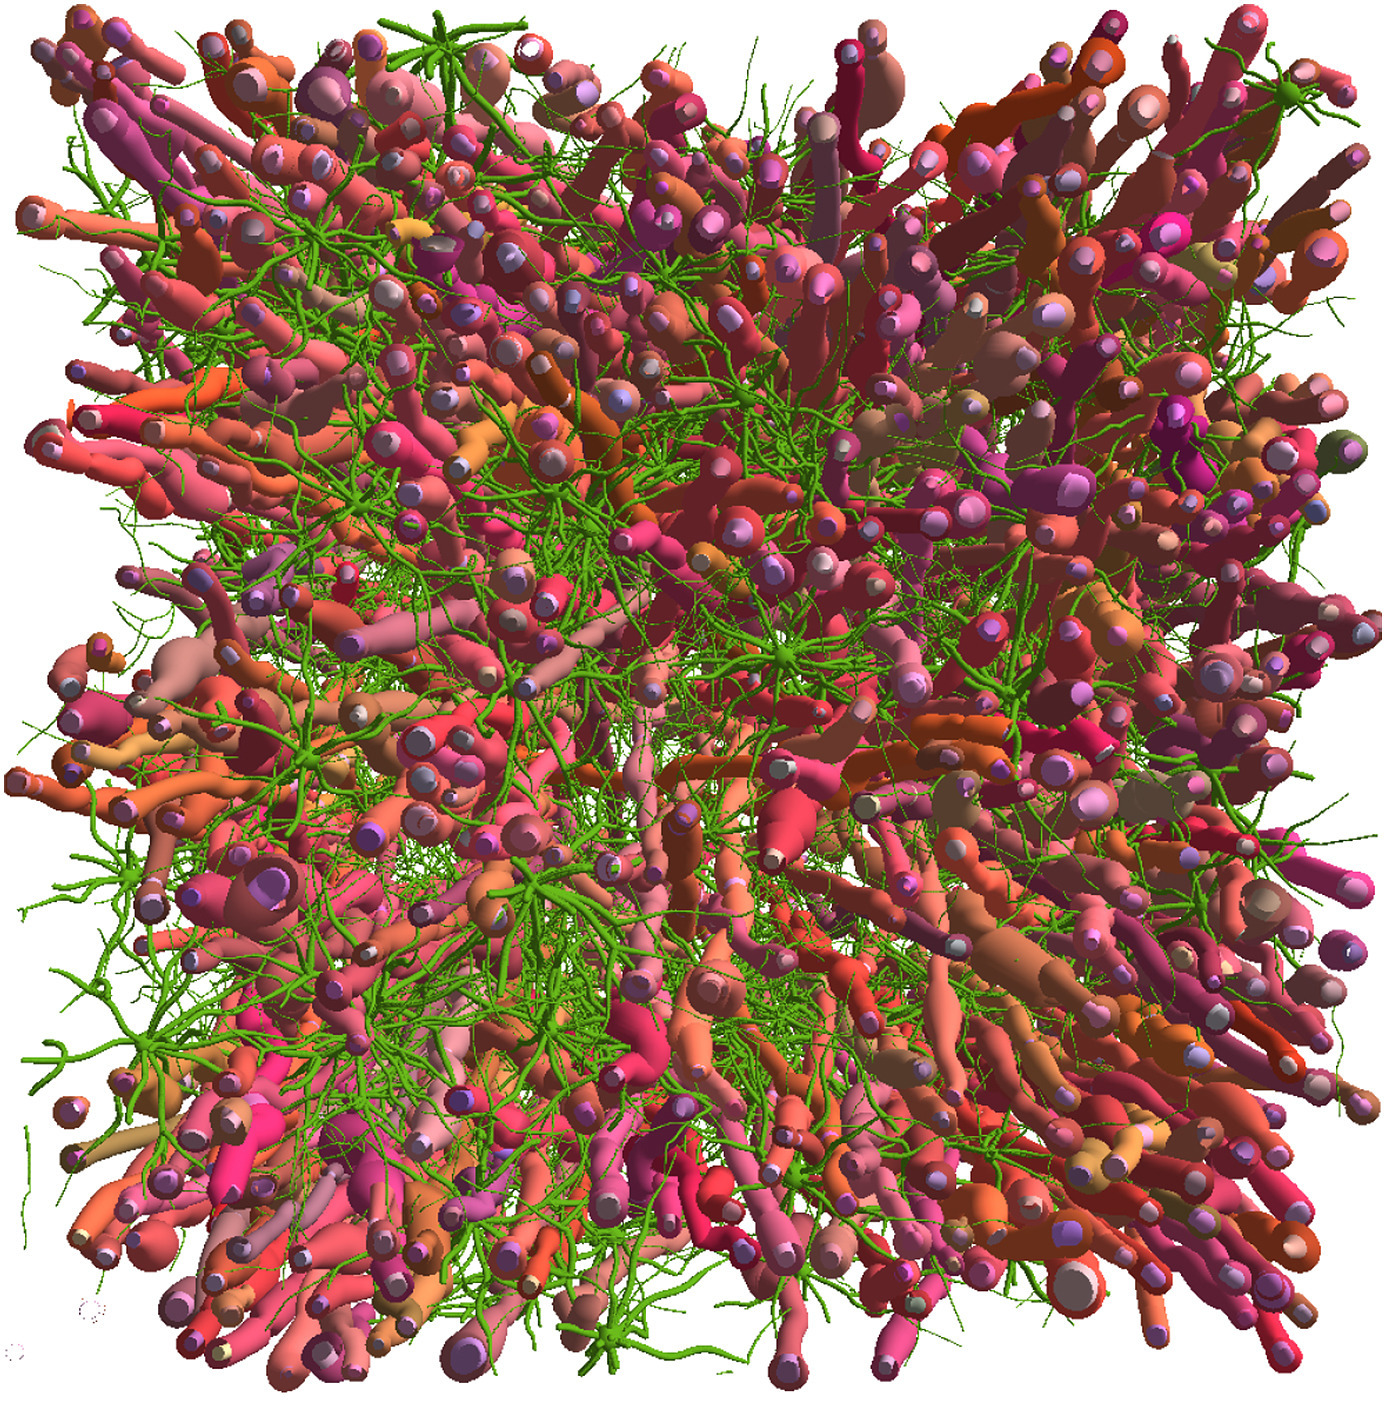
\includegraphics{gfx/model/medusa/11_.jpg}}}
	\caption{\cite{Ginsburger2019}}
	\label{fig:medusa_8}
\end{figure}
% 